\section{The System}
\label{sec.thesystem}
The system is a multi-device computing application for sharing
pictures. Its purpose is to move photo from android phones holding personal
information, to a shared/public tabletop where many  people can browse the
photos all together. \\

The main requirements are to establish a two-way communication between the
devices and remote control of the pictures on the tabletop, from the
phone. \\

At startup, the android application displays an image gallery,
from where the user can throw images to the tabletop. When the throw gesture is
detected a communication to the server (tabletop) is established. The image, on
the tabletop, can be controlled from the phone. This is realized by sending the
move coordinates using the basic message protocol. After processing the image,
this can be sent back to the phone, by performing a custom gesture. An dialog
containing the picture is displayed on the android.

\subsection{Overall System Design}
\label{sec.thesystem.design}

The overall system design is illustrated in figure \ref{fig.system_overview}.
As shown in the figure, the system is composed of a tabletop surface, which can
communicate with Android devices. A user can choose to drag and drop pictures
from the phone to the table and vice-versa.

 \begin{figure}[H]
    \begin{center}
        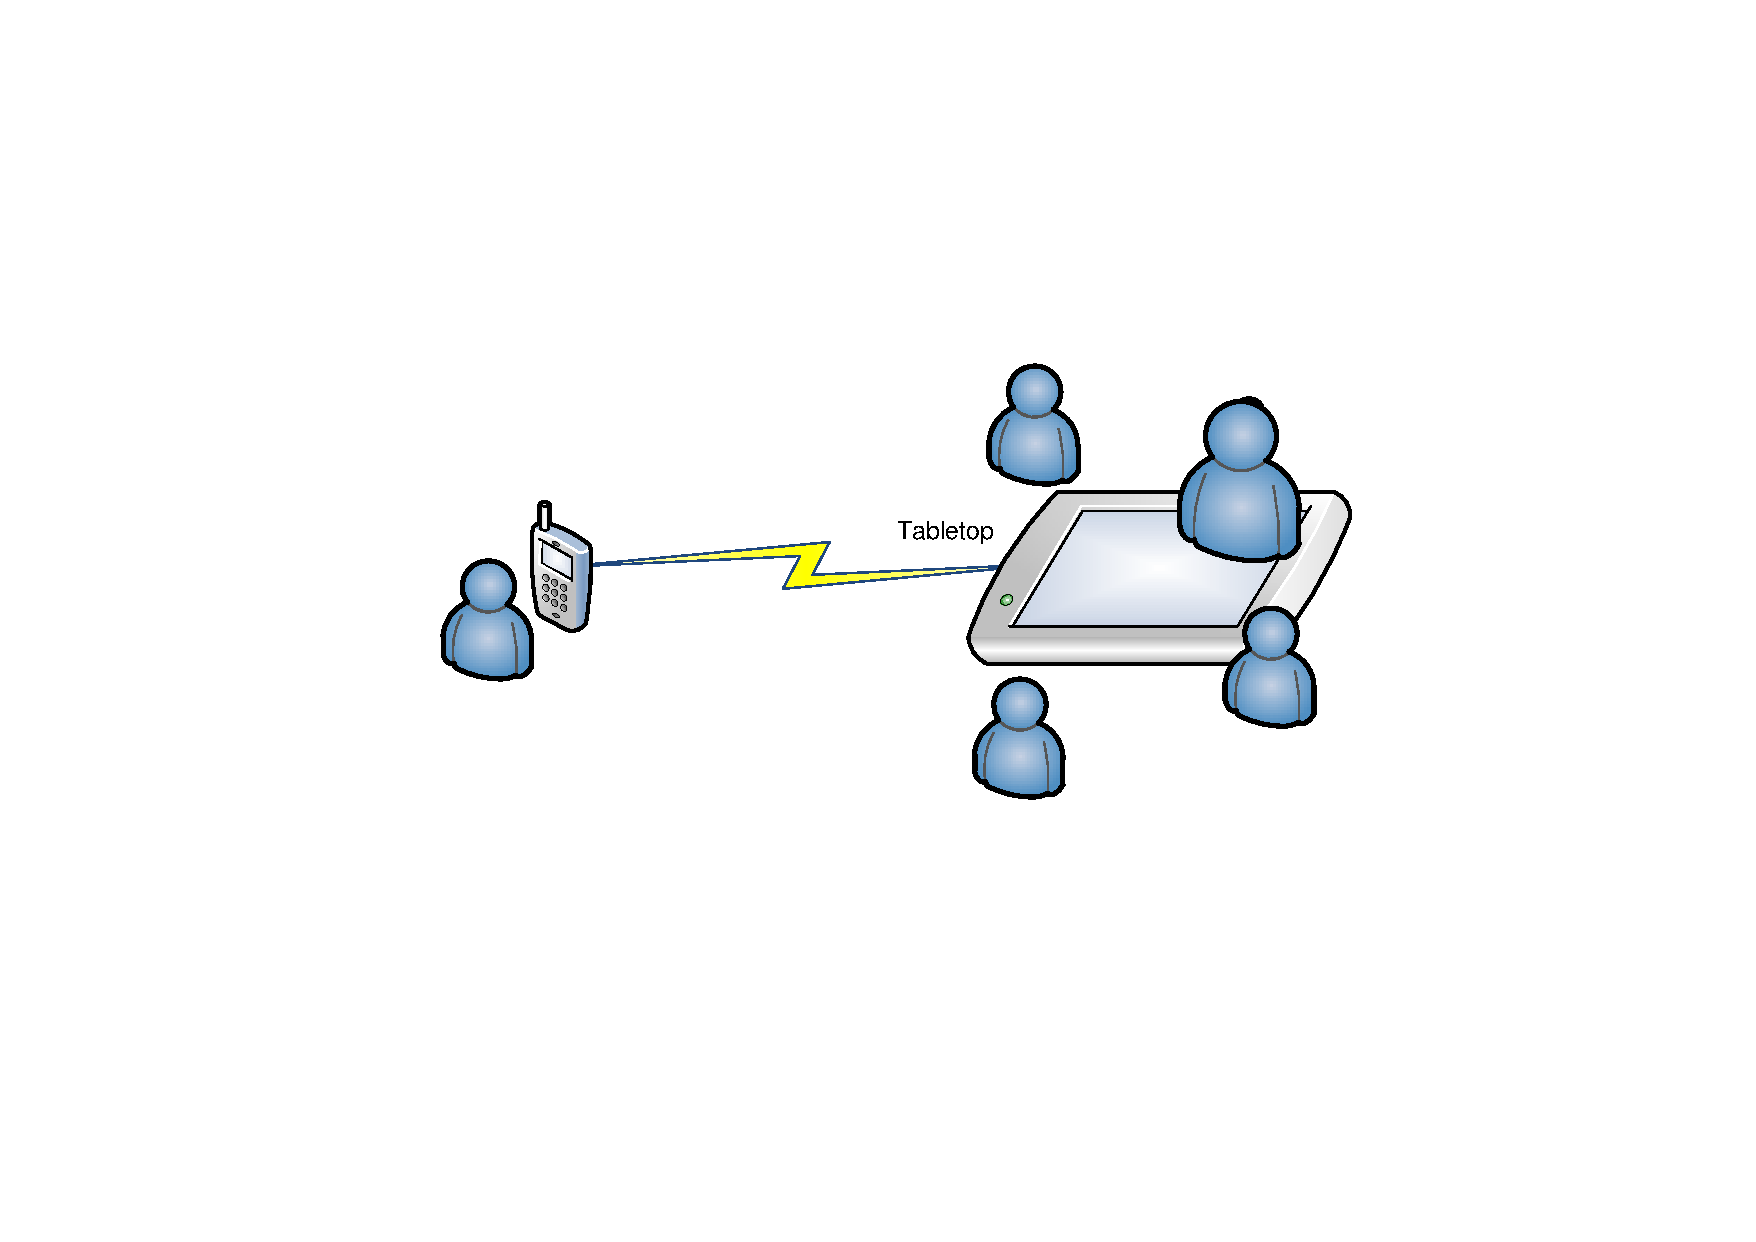
\includegraphics[width=\textwidth]{fig/system_overview.pdf}
        \caption{Overview of the System Design}
        \label{fig.system_overview}
    \end{center}
\end{figure}

\subsection{MT4J}
\label{sec.thesystem.mt4j}
MT4j\footnote{Multitouch for Java} is an open source cross-platform framework,
created for rapid development of visually rich applications. The toolkit can be
used for 2D, 3D applications and it supports different kinds of input devices with a
special focus on multi-touch support.\\

We have used the MT4J framework to develop two applications running on the
tabletop. The first application, \emph{MTTemplateCreatorApplication}, is used to
define a custom gesture. It consists of a \emph{rectangle} where the user defines the gesture, a \emph{start/stop} button
to start/stop the gesture registration, a \emph{clear} button to clear the
gesture registration area and a \emph{save} button which will save the custom
gesture in a file. The gesture is saved as a serialized object of type
\emph{ArrayList<SerializableVector3D>}.\\

The second application, \emph{MTDragDropApplication}, represents the multi-touch
and multi-user photo browsing application. At start-up, the application loads
all the images in the \emph{images} directory, reads the custom gesture from the
\emph{custom.ges} file, defines a \emph{DragDrop area} to send images back to
the client and starts up a server listening for connection. When a new image is received from the client Android application, the image is
displayed on the surface. Multiple users are now able to manipulate the client
image. When a user wants to send images back to the phone, they have to be
placed in the \emph{DragDrop area} and the send gesture has to be performed.\\

When performing the save gesture, the images were also moving on the surface.
To overcome this issue, the save operation has to be performed in two steps:
a click in the \emph{DragDrop area} will remove all gesture listeners (rotate,
drag and scale) from the images in the send area and attach the custom gesture
listener. After this step the gesture can be performed without the images
moving. A second click in the DragDrop area will remove the custom gesture
listeners from the images and re-attach the rotate, drag and scale gesture
listeners.

\subsection{Communication}
\label{sec.thesystem.communication}
A TCP/IP communication is established between the tabletop and the android
device. It is a client-server based communication: the surface is implemented
as a server, while the phone is the client. The communication happens through an
open socket between the two devices. The table top opens a ServerSocket, which
listens for requests. The android establishes the connection to the server using
its IP address and specified port number.

Both the Android device and the table top can either send or
receive pictures and coordinates.

The protocol of the communication consists in messages in the form of byte
arrays. The first byte sent stands for the operation type, which can be:       
0 = leaving; 1 = image; 2= coordinates. 
If the operation type is send image, the message has the following
structure:
\begin{itemize}
  \item 1 byte for type
  \item 1 int equal to the length of the image in bytes
  \item the actual bytes of the image in the form of array bytes
\end{itemize}
If the operation type is send image, the message has the following
structure:
\begin{itemize}
  \item 1 byte for type
  \item 1 float representing the x coordinate
  \item 1 float representing the y coordinate
\end{itemize}

The interaction and communication of the devices is depicted in the sequence
diagram from figure \ref{fig.sequence_diagram}.

 \begin{figure}[H]
    \begin{center}
        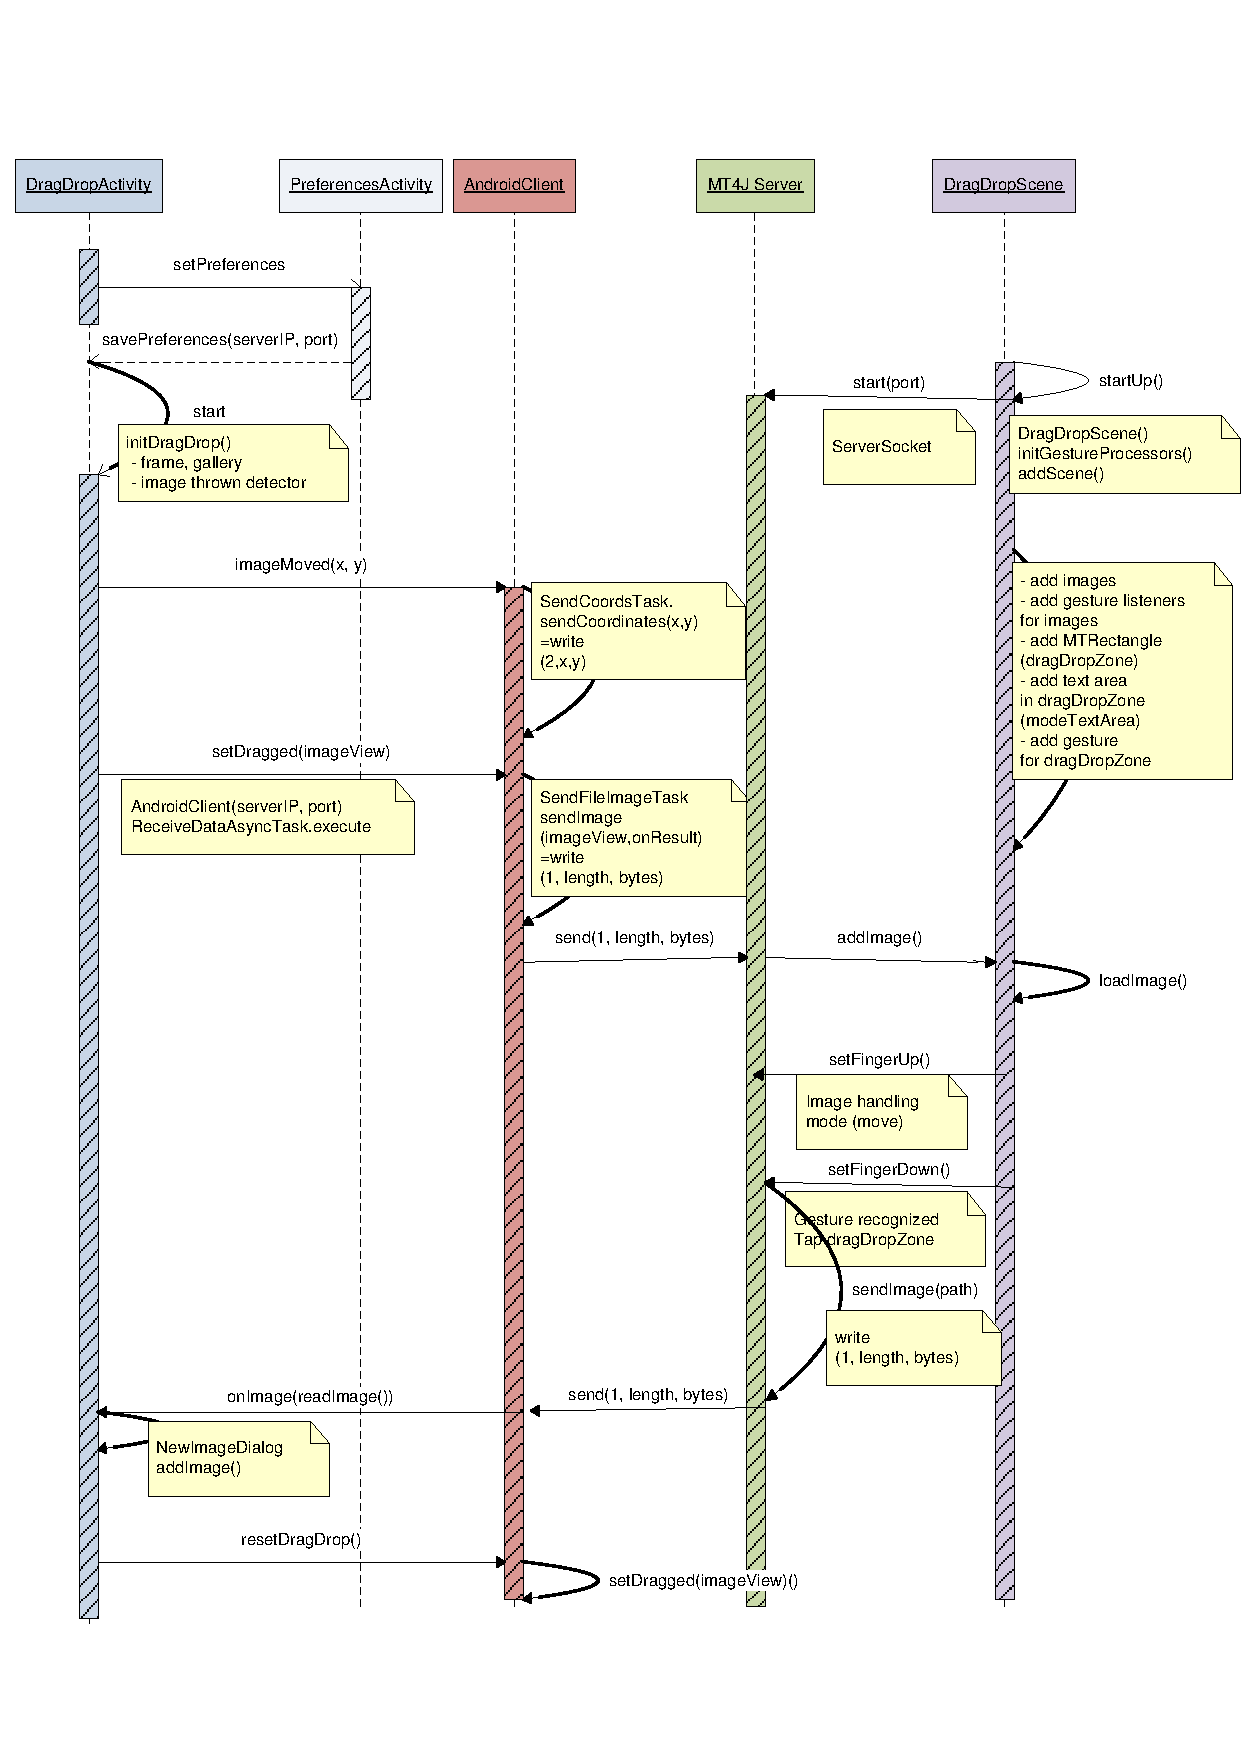
\includegraphics[width=\textwidth]{fig/sequence_diagram.pdf}
        \caption{Communication Sequence Diagram }
        \label{fig.sequence_diagram}
    \end{center}
\end{figure}
